%%%%%%%%%%%%%%%%%%%%%%%%%%%%%%%%%
% Entropy of approximate sets
%%%%%%%%%%%%%%%%%%%%%%%%%%%%%%%%%%%
\section{Entropy of approximate sets}
\label{sec:entropy}
The Bernoulli set model assigns binomial distributions to the number of false
positives and false negatives.
A natural question is how much \emph{uncertainty} these error counts carry,
as measured by Shannon entropy~\cite{shannonBSC}.
In this section, we derive the joint entropy of the false positive and false
negative counts and extend the analysis to the case in which the number of
positives is itself uncertain.

\begin{theorem}[Joint entropy of false positives and false negatives]
\label{thm:joint_entropy_fp_fn}
Given $m$ positives in a universe of $u$ elements, the joint entropy of the
uncertain number of false positives and false negatives in a Bernoulli set with
expected false positive rate $\fprate$ and expected false negative rate $\fnrate$
is
\begin{equation}
\label{eq:joint_entropy}
    \Entropy{\FP_m, \FN_m}
    = \log_2(2\pi e)
    + \frac{1}{2}\log_2\!\bigl(
        (u - m) \cdot m \cdot \fprate(1-\fprate) \cdot \fnrate(1-\fnrate)
      \bigr)
    + \mathcal{O}\!\left(\frac{u}{m(u-m)}\right).
\end{equation}
\end{theorem}
\begin{proof}
By \cref{asm:element_indep}, the random error counts $\FP_m$ and $\FN_m$
are conditionally independent given $m$ positives (they are functions of
indicators on disjoint element sets: negatives and positives respectively).
Therefore the joint entropy decomposes additively:
\begin{equation}
    \Entropy{\FP_m, \FN_m} = \Entropy{\FP_m} + \Entropy{\FN_m}.
\end{equation}
The random variable $\FP_m$ is binomially distributed,
$\FP_m \sim \operatorname{Bin}(u - m,\, \fprate)$.
The entropy of a binomial distribution $\operatorname{Bin}(n, p)$ admits the
well-known asymptotic expansion~\cite{coverThomas}
\begin{equation}
\label{eq:binomial_entropy_asymp}
    H = \frac{1}{2}\log_2\!\bigl(2\pi e \cdot n \cdot p(1-p)\bigr)
      + \mathcal{O}(1/n).
\end{equation}
Applying \cref{eq:binomial_entropy_asymp} to $\FP_m$ and $\FN_m$ respectively
yields
\begin{align}
    \Entropy{\FP_m}
    &= \frac{1}{2}\log_2(2\pi e)
     + \frac{1}{2}\log_2\!\bigl((u-m)\,\fprate(1-\fprate)\bigr)
     + \mathcal{O}\!\left(\frac{1}{u-m}\right), \\
    \Entropy{\FN_m}
    &= \frac{1}{2}\log_2(2\pi e)
     + \frac{1}{2}\log_2\!\bigl(m\,\fnrate(1-\fnrate)\bigr)
     + \mathcal{O}\!\left(\frac{1}{m}\right).
\end{align}
Summing these expressions and combining the logarithms gives
\begin{equation}
    \Entropy{\FP_m, \FN_m}
    = \log_2(2\pi e)
    + \frac{1}{2}\log_2\!\bigl(
        (u-m)\, m\, \fprate(1-\fprate)\, \fnrate(1-\fnrate)
      \bigr)
    + \mathcal{O}\!\left(\frac{u}{m(u-m)}\right),
\end{equation}
where the error term follows from
$\mathcal{O}(1/(u-m)) + \mathcal{O}(1/m)
 = \mathcal{O}\!\bigl(u / (m(u-m))\bigr)$.
\end{proof}

\subsection{Positives and negatives}
\label{sec:entropy:pos_neg}
When the number of positives is itself uncertain, modeled by the random
variable $\POS$ with probability mass function $\Fun{p}_{\POS}(p \Given u)$,
the joint distribution of positives, false positives, and false negatives
factorizes as
\begin{equation}
\label{eq:joint_pos_fp_fn}
    \Fun{p}(p, f_p, f_n \Given u, \fprate, \fnrate)
    = \Fun{p}_{\POS}(p \Given u)
      \;\Fun{p}_{\FP}(f_p \Given p, u, \fprate)
      \;\Fun{p}_{\FN}(f_n \Given p, u, \fnrate).
\end{equation}
By \cref{asm:element_indep}, $\FP$ and $\FN$ are conditionally independent
given $\POS$, so the joint entropy decomposes as
\begin{equation}
\label{eq:joint_entropy_pos}
    \Entropy{\POS, \FP, \FN}
    = \Entropy{\POS}
    + \sum_{p=0}^{u} \Fun{p}_{\POS}(p \Given u)\, \Entropy{\FP \Given p}
    + \sum_{p=0}^{u} \Fun{p}_{\POS}(p \Given u)\, \Entropy{\FN \Given p}.
\end{equation}
The last two sums are the conditional entropies $\Entropy{\FP \Given \POS}$
and $\Entropy{\FN \Given \POS}$, each weighted by the distribution of
positives.

\begin{example}
The \emph{expected} number of false positives, marginalizing over $\POS$, is
\begin{align}
    \Expect{\FP}
    &= \sum_{p=0}^{u} \Fun{p}_{\POS}(p \Given u)\, \Expect{\FP_p}
     = \sum_{p=0}^{u} \Fun{p}_{\POS}(p \Given u)\, (u - p)\,\fprate \notag \\
    &= \fprate \bigl(u - \Expect{\POS}\bigr)
     = \fprate \cdot \Expect{\NEG},
\end{align}
confirming that the marginal expected false positive count depends only on the
expected number of negatives and the false positive rate $\fprate$.
\end{example}

\subsection{Space complexity}
\label{sec:space_comp}
If the finite cardinality of a universe is $u$ and the set is \emph{dense} (and the approximation is also dense, i.e., the false negative rate is relatively
small), then
\begin{equation}
    \mathcal{O}(u) \; \si{bits}
\end{equation}
are needed to code the set, which is independent of $\p$, the false positive rate, and the false negative rate.

The lower-bound on the \emph{expected} space complexity of a data structure that models the \emph{positive random approximate set} where the elements are over a \emph{countably infinite} universe is a classical result due to Carter, Floyd, Gill, Markowsky, and Wegman~\cite{carterExact}.
We restate it here in the notation of the present paper and include a proof for completeness.
\begin{proposition}[{\cite{carterExact}}]
\label{pst:approx_l_b}
The \emph{information-theoretic lower-bound}\index{information-theoretic lower-bound} of a data structure that implements the countably infinite \emph{positive random approximate set} abstract data type has an \emph{expected} bit length given by
\begin{equation}
    -\log_2 \fprate \; \si{bits \per element},
\end{equation}
where $\fprate > 0$ is the false positive rate\index{false positive rate}.
\end{proposition}
\begin{proof}
It suffices to prove the bound for deterministic encodings; the extension to randomized data structures follows from Yao's minimax principle.

Consider a finite subset of the universe with $n$ elements, from which an
objective set $S$ of size $\p$ is drawn.
A deterministic encoding using $B$ bits maps each input set $S$ to a state
$r = f(S)$ from at most $2^B$ distinct states.
Each state $r$ determines a \emph{positive response set}
$Q(r) = \{x : \text{query}(x,r) = 1\}$.
Since the data structure has no false negatives ($\tprate = 1$), we have
$S \subseteq Q(r)$ for the state $r = f(S)$ encoding $S$.
The false positive rate constraint requires that at most an $\fprate$-fraction of the $n - \p$ negatives belong to $Q(f(S))$ for every input set $S$, so
$|Q(f(S))| \leq \p + \fprate(n - \p)$ for all $S$.
In particular, $|Q(r)| \leq \p + \fprate(n - \p)$ for every state $r$ in the image of $f$.

By the pigeonhole principle, some state $r^*$ must encode at least
$\binom{n}{\p} / 2^B$ distinct input sets.
Every such set is a subset of $Q(r^*)$ of size $\p$, so
\begin{equation}
\binom{n}{\p} / 2^B
    \leq \binom{|Q(r^*)|}{\p}
    \leq \binom{\p + \fprate(n - \p)}{\p}.
\end{equation}
Taking logarithms and rearranging:
\begin{equation}
B \geq \log_2 \binom{n}{\p} - \log_2 \binom{\p + \fprate(n - \p)}{\p}.
\end{equation}
For fixed $\p$ as $n \to \infty$, $\binom{n}{\p} \sim n^\p / \p!$ and
$\binom{\p + \fprate n}{\p} \sim (\fprate n)^\p / \p!$, so
\begin{equation}
B \geq \log_2 \frac{n^\p}{(\fprate n)^\p}
    = \p \log_2 \frac{1}{\fprate}
    = -\p \log_2 \fprate,
\end{equation}
giving $-\log_2 \fprate$ bits per element.
\end{proof}
\begin{remark}
\label{rem:general_lower_bound}
The general case $0 < \tprate < 1$ remains open.
When false negatives occur, $S \not\subseteq Q(r)$ and the pigeonhole step
above fails: valid input sets are no longer constrained to be subsets of the
positive response set.
The heuristic scaling $-\tprate \log_2 \fprate$ (retaining $\p \tprate$
elements on average, each requiring $-\log_2 \fprate$ bits) is plausible
but is not a valid information-theoretic lower bound, since the encoding
problem changes qualitatively when elements are randomly dropped.
\end{remark}

A well-known implementation of countably infinite \emph{positive approximate set} is the Bloom filter~\cite{bf} which has an expected space complexity given
by
\begin{equation}
    -\frac{1}{\ln 2} \log_2 \fprate \; \si{bits \per element},
\end{equation}
thus the absolute efficiency of the Bloom filter is $\ln 2 \approx 0.69$.
A practical implementation of the \emph{positive random approximate set} is given by the \emph{Perfect Hash Filter}~\cite{phf}, which compares favorably to the Bloom filter in many circumstances.\footnote{The \emph{Singular Hash Set}~\cite{shs} is an example of a data structure that obtains optimality using \emph{brute-force} search, so it is not practical for even relatively small objective sets. However, its primary purpose is analytic tractability.}

\begin{figure}[ht]
\centering
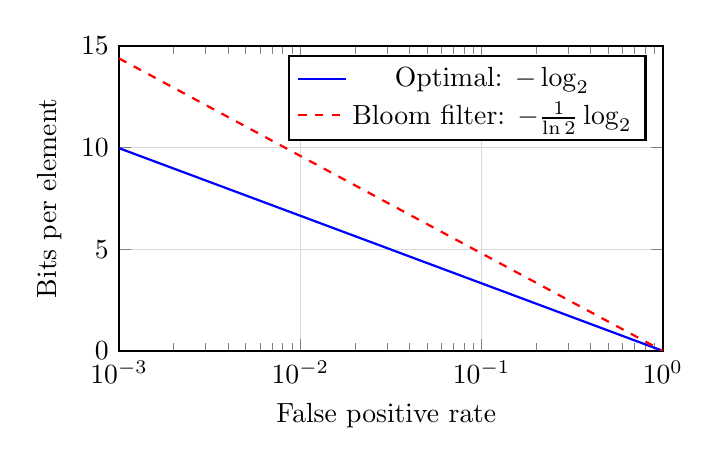
\begin{tikzpicture}
\begin{axis}[
	width=0.7\textwidth,
	height=0.45\textwidth,
	xlabel={False positive rate $\fprate$},
	ylabel={Bits per element},
	xmin=0.001, xmax=1,
	ymin=0, ymax=15,
	xmode=log,
	legend pos=north east,
	ymajorgrids, xmajorgrids,
	major grid style={gray!30},
	thick,
	samples=200,
	domain=0.001:1,
]
\addplot[blue, solid] {-ln(x)/ln(2)};
\addlegendentry{Optimal: $-\log_2 \fprate$}
\addplot[red, dashed] {-ln(x)/ln(2)/ln(2)};
\addlegendentry{Bloom filter: $-\frac{1}{\ln 2}\log_2 \fprate$}
\end{axis}
\end{tikzpicture}
\caption{Space complexity of positive approximate sets as a function of
the false positive rate $\fprate$.
The solid curve is the information-theoretic lower bound
$-\log_2 \fprate$ bits per element (\cref{pst:approx_l_b}).
The dashed curve is the Bloom filter cost
$-(1/\ln 2)\log_2 \fprate$; the gap reflects the Bloom filter's
$\ln 2 \approx 69\%$ efficiency.}
\label{fig:space_lower_bound}
\end{figure}
